% LLNCStmpl.tex
% Template file to use for LLNCS papers prepared in LaTeX
%websites for more information: http://www.springer.com
%http://www.springer.com/lncs
\documentclass{llncs}

\usepackage{graphicx}
\usepackage{float}
\usepackage{hyperref}
\usepackage{listings}

\begin{document}
\title{Linux client with WiFi and LTE}
\subtitle{Project report}
\author{Pascal Maissen, Jovana Micic, Noe Wysshaar} 
\institute{University of Bern\\  \email {pascal.maissen@unifr.ch, jovana.micic@students.unibe.ch, noemathieu.wysshaar@unifr.ch} }
\maketitle

%Maximum 2 pages about the theoretical basics of the experiment.
\section{Protocol Introduction}
The task of this project is study of Dynamic Adaptive Streaming over HTTP video delivery in a mobile scenario using WiFi and Long Term Evolution (LTE). Case scenario is that the user is connected through LTE, but periodically gets the internet access through WiFi. The main goal of this project is to evaluate the quality gain in the parallel LTE/WiFi video transmission in comparison to a single LTE transmission using multi-path TCP (MPTCP).

In order to achieve parallel connection of LTE and WiFi we have to use MPTCP. Multi-path TCP is a  recent attempt  to handle simultaneous use of multiple paths at the transport layer \cite{MPTCP}. The core idea of MPTCP is to define a way to build a connection between two hosts and not between two interfaces (as standard TCP does). MPTCP represents the evolution of TCP protocol and it works in all networks where TCP works.  Benefits of MPTCP include better resource utilization, better throughput and smoother reaction to failures. Using MPTCP dramatically improves Quality of Experience of video streaming. 

\begin{figure}[H]
\centering
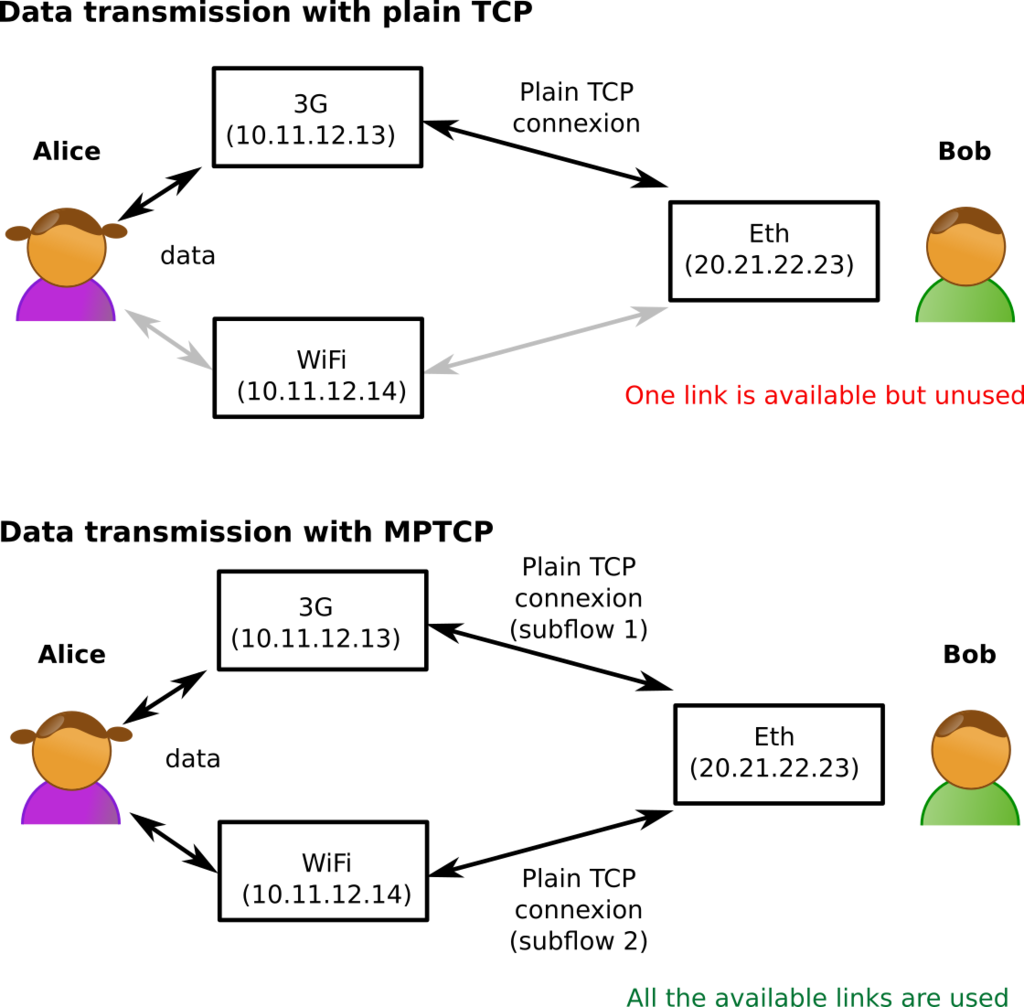
\includegraphics[width=0.5\textwidth]{mptcp.png}
\caption{\label{fig:mptcp} Difference between TCP and MPTCP.}
\end{figure}

In the figure \ref{fig:mptcp} is presented graphic explaining the difference between TCP and MPTCP.  For instance, Alice has a smartphone with 3G and WiFi interfaces and Bob has a computer with an Ethernet interface. In standard TCP, the connection should be established between two IP addresses. An application can only create one TCP connection through a single link. MPTCP allows the connection to use several paths simultaneously. For this, MPTCP creates one TCP connection, subflow, over each path that needs to be used. So in the case from the figure \ref{fig:mptcp},  Alice can use both available links, 3G and WiFi at the same time.

In our project description it was required to use Dynamic Adaptive Streaming over HTTP (DASH). DASH is a streaming technique that enables high quality streaming of media content over the Internet \cite{DASH}. DASH works by breaking the content into a sequence of small HTTP-based file segments, each segment containing a short interval of playback time of content that is potentially many hours in duration, such as a movie or the live broadcast of a sports event. The content is made available at a variety of different bit rates, i.e., alternative segments encoded at different bit rates covering aligned short intervals of playback time. DASH client can adapt to changing network conditions and provide high quality playback with fewer stalls or re-buffering events. DASH should not be confused with a transport protocol, the transport protocol that DASH uses is TCP.

\begin{figure}[H]
\centering
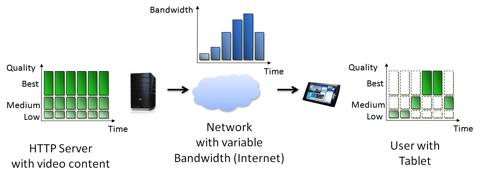
\includegraphics[width=1.0\textwidth]{DASH.png}
\caption{\label{fig:dash} Concept of Dynamic Adaptive Streaming over HTTP.}
\end{figure}

In the figure \ref{fig:dash} is presented concept of DASH. This concept is consisting of the three parts. First part is HTTP server with video content of different qualities. Second part is network which has varying bandwidth conditions. Third part is user with device which selects appropriate segments for each timepoint. So the main advantage of using DASH is that is flexible, it dynamically adapts to current network conditions and it reuses existing Internet architecture.

%The experimental setup, the differences of the experimental series, the different parameters used.
\section{Experimental setup}
For MPTCP to work we needed to install the MPTCP kernel \cite{linuxMPTCP}.
We downloaded, compiled and installed the kernel on two linux machines. One later acting as client and the other one as server. The setup is illustrated on figure \ref{fig:setup}.\\


\begin{figure}[H]
\centering
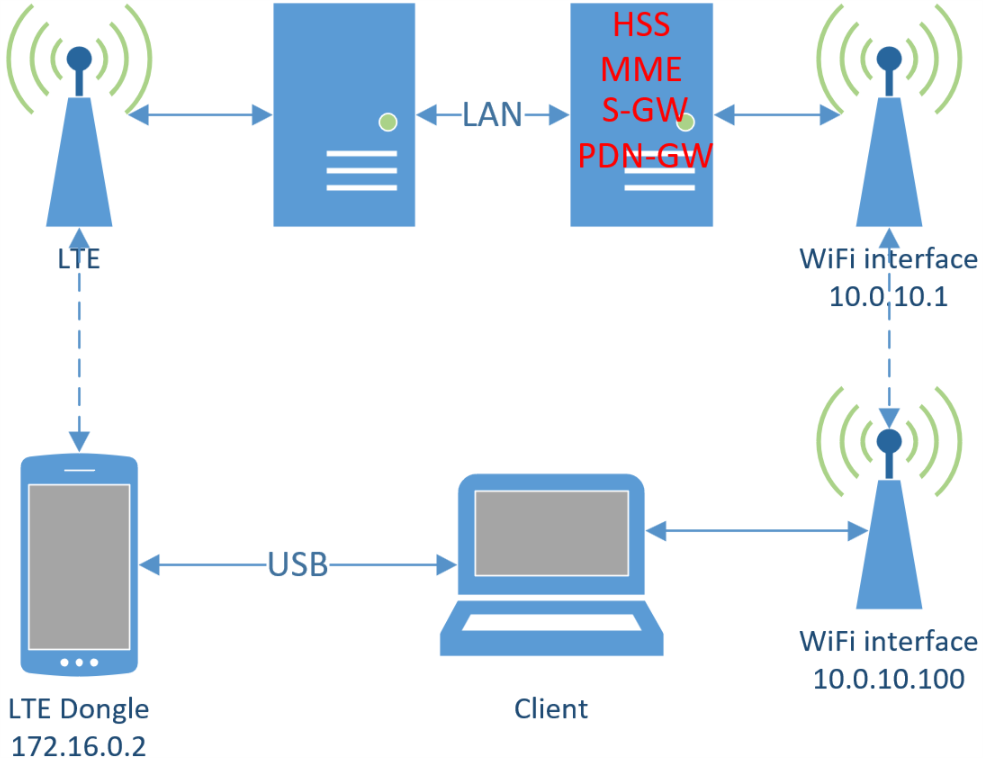
\includegraphics[width=0.8\textwidth]{setup.png}
\caption{\label{fig:setup} Hardware setup used for the experiments.}
\end{figure}

Both computers needed at least two network interfaces. The client was equipped with a wireless network card for the WiFi connection and for the connection over LTE we used a USB dongle. On the serverside a custom WiFi access point was created with the help of hostapd \footnote{hostapd \url{http://w1.fi/hostapd/}} to which the client connected. In addition, the server needs to be connected with an LTE antenna. To our luck this computer was already set up for this task and had all necessary LTE components such as the Home Subscriber Server (HSS), Mobility Management Entity (MME), Serving Gateway (S-GW) and PDN Gateway (P-GW). Among some minor diffuculties regarding the establishment of the LTE connection (presumably
 due to a poor LTE dongle) everything was set up and ready for testing.\\

In the first part of our experiment we just tested throughput of the data without video streaming. We had two different scenarios:

\begin{enumerate}
\item{LTE and WiFi working in parallel. WiFi was turned off after 10 seconds and then turned on after 10 seconds.}
\item{WiFi was turned off and LTE was on. WiFi was turned on after 10 seconds.}
\end{enumerate}

In the second part of our experiment we wanted to test data throughput in a scenario when user is watching a video content from the Internet. So the first step was to find appropriate video which we will stream over the Internet. Appropriate video means that bitrate of the video has to be larger than 25 Mbps because of the  restulst we got in the first experiment. We choose \emph{4K Ultra HD Firework }video\footnote{Firework video \url{http://4ksamples.com/4k-uhd-fireworks-sample/}}. In the table \ref{tab:video} is presented general information about video. 

\begin{table}
\centering
\begin{tabular}{l|l}
Attribute & Value \\\hline
Format & MPEG-4 \\
File size & 1.19 GiB \\
Duration & 1mn 47s \\ 
Overall bitrate & 95.7 Mbps \\
Width & 3 840 pixels \\
Height & 2 160 pixels \\
Writing library \hspace{10mm}  &  x264 core 114 \\
\end{tabular}
\caption{\label{tab:video}General information about video.}
\end{table}

The next step was to prepare video for DASH streaming. We encoded a video in different qualities to provide multiple representations according to the DASH standard. For transcoding the video to the H.264 standard we used x264 library\footnote{x264 \url{https://www.videolan.org/developers/x264.html}}. This library is a free software library for encoding video streams into the H.264/MPEG-4 AVC compression format. Example of the shell script used for creating video of 5 Mbps bitrate is presented in the following listing.

\begin{lstlisting}[language=bash, caption={\label{l:script}Shell script for encoding the video.}, captionpos=b]
bitrate=5000

x264 --output intermediate_${bitrate}k.264 --fps 60 --preset
slow --bitrate $((bitrate)) --vbv-maxrate $((bitrate*2)) 
--vbv-bufsize $((bitrate*2*2)) --min-keyint 120 --keyint 120 
--scenecut 0 --no-scenecut --pass 1 
--video-filter "resize:width=1280,height=720" firework.mp4

MP4Box -add intermediate_${bitrate}k.264 -fps 60
out_${bitrate}k.mp4 rm intermediate_${bitrate}k.264

\end{lstlisting} 

Output of this script is a raw H.264 video which data is encapsulated in a mp4 container. MPEG-4 Part 14 or mp4 is a digital multimedia container format most commonly used to store video and audio. Using script presented in the listing, we created different representations. Description of all representations is presented in the table \ref{tab:repr}.

\begin{table}
\centering
\begin{tabular}{c|c|c}
Representation ID & Resolution [px x px] & Bitrate [Mbps] \\\hline
1 & 1280 x 720 & 5 \\
2 & 1280 x 720 & 10 \\
3 & 1920 x 1080 & 15 \\
4 & 1920 x 1080 & 20 \\
5 & 1920 x 1080 & 25 \\
\end{tabular}
\caption{\label{tab:repr}The different representations of the encoded video.}
\end{table}

We choose this range of bitrates because we want to be sure that we will use different representations during the streaming depending on that if we use only LTE or WiFi and LTE in parallel. After we created all representations, the next step was to "dashify" the content so it is appropriate for the DASH protocol. For that purpose we used MP4Box\footnote{MP4Box \url{https://gpac.wp.imt.fr/mp4box/}}, multimedia packager available in GPAC. It is used for performing  manipulations on multimedia files like AVI, MPG, TS, but mostly on ISO media files (e.g. MP4, 3GP). In the following listing is presented a command used for "dashifying" content.

\begin{lstlisting}[language=bash, caption={\label{l:command}Command for dashyfing content using MP4Box.}, captionpos=b]

MP4Box -dash ts -frag ts -rap -out DASHFILE.mpd 
-profile live VIDEO_QUALITY1.mp4 VIDEO_QUALITY2.mp4 ...
\end{lstlisting} 

The most important file of previous process is \emph{DASHFILE.mpd}, created manifest, which is needed for the stream itself. Media presentation description (MPD) describes segment information. It is an XML document describing where the various media resources present in the content are located. The segment is  a continuous part of a media resource. The segment is the smallest part of the media that can be located in the MPD. All produced content, including the MPD manifest, we store on the university Apache server. After that we were able to run the experiment and measure data.

For playing the video, we used MP4Client\footnote{MP4Client \url{https://gpac.wp.imt.fr/player/}}. It is provided by GPAC\footnote{GPAC \url{https://gpac.wp.imt.fr/}} and it is a highly configurable multimedia player. It can be used from a command-line, as a GUI or browser plugin. In our experiment we used it from command-line, running the command presented in the following listing.

\begin{lstlisting}[language=bash, caption={\label{l:cmd}Command for running MP4Client player.}, captionpos=b]

MP4Client <server_address>/DASHFILE.mpd

\end{lstlisting} 

We used Wireshark for capturing the data. In the second experiment, we had only one scenario where LTE and WiFi were active from the beginning. After 20 seconds, we turned off WiFi and after 20 seconds, turned on WiFi. 

%Analyze your data with respect to the aim of the experiment. Your task during the experiment is not just to measure and document your measurements, but to derive and present conclusions from your measurements. If there are some errors in the final results. Investigate and try to understand all types and sources of errors in all your measurements.
\section{Results and Analsys}
As it was mentioned in the previous section, for the first part of the project we measure data throughput for the two case scenarios. In the following text we will present results we got from this experiments.

\begin{figure}
\centering
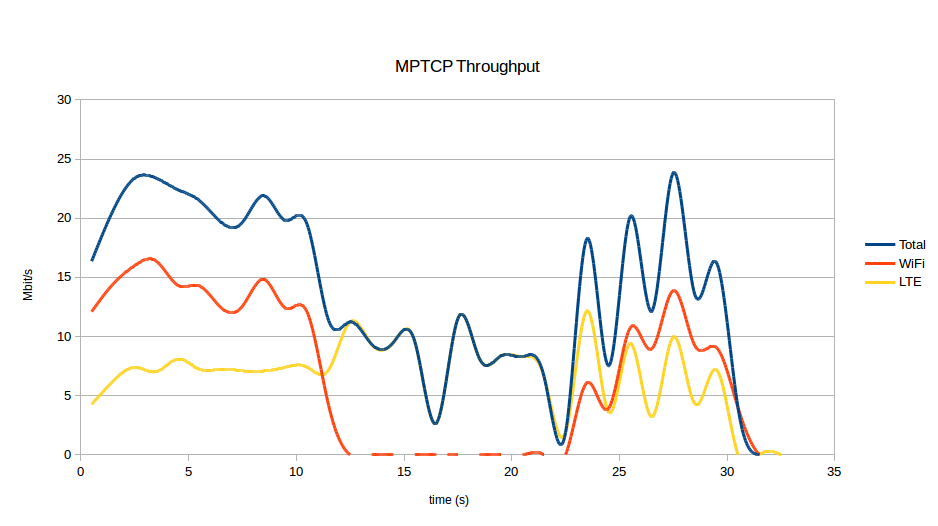
\includegraphics[width=1.0\textwidth]{result1.png}
\caption{\label{fig:r1} Graphic representing the MPTCP throughput when WiFi is turned off after 10 sec.}
\end{figure}

In the figure \ref{fig:r1} is presented throughput in the scenario when we have in parallel WiFi and LTE from the beginning of the experiment. After 10 seconds, we turned off WiFi. As we can see from the graphic, LTE continues to work but total throughput becomes lower and equal as LTE throughput. After 10 seconds, we had again turned WiFi on and it can be seen clearly on the figure that we have some WiFi throughput after 20 seconds. The maximal total throughput achieved in this scenario is around 24 Mbps.

\begin{figure}
\centering
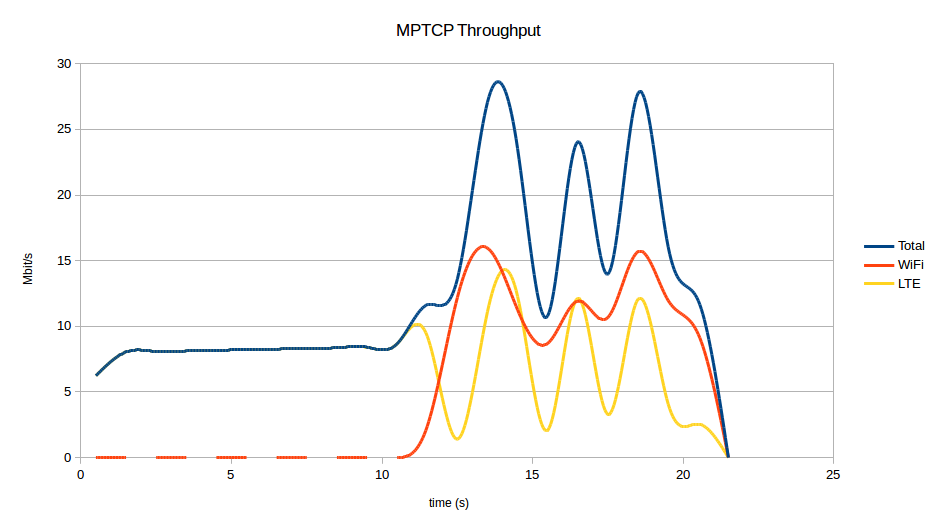
\includegraphics[width=1.0\textwidth]{result2.png}
\caption{\label{fig:r2} Graphic representing the MPTCP throughput when WiFi is turned on after 10 sec.}
\end{figure}

In the figure \ref{fig:r2} is presented throughput in the scenario when only LTE is turned on from the beginning of the experiment. After 10 seconds, WiFi is turned on. From the graphic we can see that there is increase of total throughput when WiFi is on. The maximal total throughput achieved in this scenario is around 28 Mbps.

The interesting observation from both graphics is that in the moment when the WiFi is again turned on, we have decrease of the LTE throughput. Reason for this could be specific MPTCP protocol implementation but we can not claim this with great certainty.

 
\begin{figure}[H]
\centering
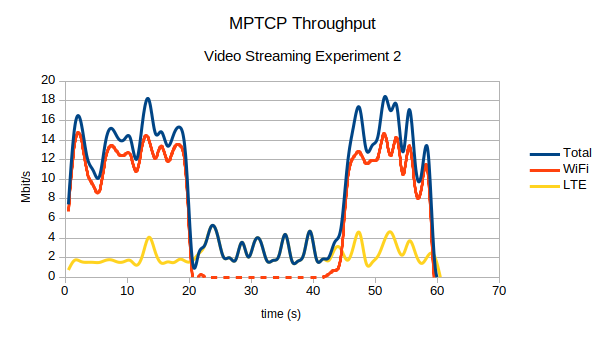
\includegraphics[scale=0.8]{videotest2.png}
\caption{\label{fig:videotest2} Throughput of MPTCP over LTE and WiFi.}
\end{figure} 
 
Figure \ref{fig:videotest2} shows the throughput of both network interfaces during a DASH video streaming test. At the start both interface are active and after 20 seconds WiFi was turned off (to simulate a signal loss) and around 20 seconds later on it was turned back on again. The graph shows a throughput around a relatively constant 3 Mbps for LTE. For the WiFi interface the throughput is around 12 Mbps while it is active. Overall this sums up to a total throughput around 15 Mbps with both interfaces active.

%\newpage
In the following is presented a graphic showing the change of the buffer size during the video streaming. In the figure \ref{fig:buffer2} we can see that at the beginning we are using the lowest representation but after the few seconds we came to the representation 3 because we have WiFi and LTE working in parallel. Significant drop on the graphic is because it is a moment when WiFi was turned off, so it has to adjust to new network conditions and continue playing the lowest representation. After 20 seconds, we again turned on WiFi and we can see that higher representations are used again. 

 
\begin{figure}[H]
\centering
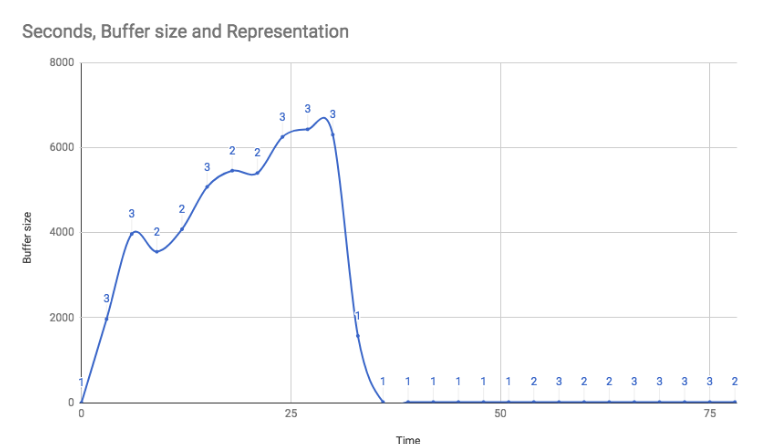
\includegraphics[width=1.0\textwidth]{buffer-test-2.png}
\caption{\label{fig:buffer2} Graphic representing the change of buffer size during the experiment.}
\end{figure}

Interesting observation in this case is that we never used representations 4 and 5. It is because we never reached bandwidth larger than 20 Mbps. Representation 4 has bitrate of 20 Mbps and representation 5 has 25 Mbps. Maybe if we run more experiments, it could happen to have larger total bandwidth, so it could use representations 4 and 5.


%Summarize and discuss your results with respect to the literature or your own scientific expectations. You should in particular discuss possible error sources and give a short judgment on the quality of the experimental setup (because you also learn to design the measurement setups). If needed, suggest how to improve the setups.
\newpage
\section{Conclusions}
The two main problems of the streaming video content are quality and buffering. For example, video that is only 1280 x 720 will never play at correct quality levels on a screen that is 1920 x 1080 px, it will be stretched. Second thing is  buffering. If the users has a poor quality internet connection, and cannot download the video stream quickly enough, then the video will need to pause, wait for more data, and then start again. This makes watching a video horrible for the user. Solution for this problem is adaptive streaming. 

Adaptive streaming allowed us to create a different video representations so we can stream a specific video file ensuring that the viewer always receives a video that will look good. Because adaptive streaming adapts to the speed of the user’s internet connection, we avoided pausing the video because of the buffering.

In our experiment we came to the conclusion that using WiFi when is available, improves the quality of experience very much. It allows user to watch video in higher resolution without pausing and waiting to buffer more data. But still, this approach is not so widely supported. We had difficulties to find appropriate resources and tutorials. Setting up this configuration would be very hard if we did not have help of Dr. Eryk Schiller, so we would like to thank him for helping us with setting everything up. 

The best achievement is that we have proven by our measurements that  the change of representation is actually happening, as it can be see on the figure \ref{fig:buffer2}. Comparing to the figure \ref{fig:videotest2}, we see that at the beginning, in the first 20 seconds, when the total throughput is between 10 and 18 Mbps, it use representations 2 and 3. After turning off WiFi, it uses only the lowest, representation 1. It is because total throughput was below 5 Mbps. In this way, user did not experience buffering of the video, because segments were already loaded in the buffer and lower representation is used. After we turned on WiFi again, we have increase of total throughput and change of the representation, higher representations are used again. 

In a previous setup where we used the Swisscom mobile LTE network and the university network \emph{eduroam}. But in this case MPTCP was not used over eduroam, while on the Swisscom LTE network it worked well. We assume this is due to firewalls settings and/or Network Address Translation (NAT). In the captured traffic there where no indications why MPTCP was not used. On the start of the experiment just a normal TCP connection was established. This meant sending traffic over both interfaces in a dynamic way was not possible.

There are still some open questions we found out during this research. One of the question is the moment when we turn on WiFi. In that moment, we have the decrease of the LTE throughput. We suppose that it has something to do with the MPTCP protocol implementation. This could be a interesting task for some further research.


%The bibliography, done here without a bib file
%This is the old BibTeX style for use with llncs.cls
\bibliographystyle{splncs}
\begin{thebibliography}{1}
%add each reference in here like this:
\bibitem{MPTCP}
Barré, Sébastien. \emph{"Implementation and assessment of modern host-based multipath solutions." } Universite catholique de Louvain, Louvain-la-Neuve, Belgium (2011).

\bibitem{DASH}
Michalos, M. G., S. P. Kessanidis, and S. L. Nalmpantis. \emph{"Dynamic Adaptive Streaming over HTTP."} Journal of Engineering Science \& Technology Review 5.2 (2012).

\bibitem{linuxMPTCP}
C. Paasch, S. Barre, et al.. \emph{Multipath TCP in the Linux Kernel}. Available from \url{http://www.multipath-tcp.org}.

%\bibitem{VLC}
%\emph{VLC player}. Available from \url{download.videolan.org/pub/videolan/vlc/2.1.0/}.

\end{thebibliography}

\end{document}

